% ============================================================
%  A GIS-based Framework for Urban Traffic CO2 Simulation
%  Le Marrec, Nguyen Gia Trong, Gascard — 2026
%  Compiled with pdflatex (requires bibtex / biblatex optional)
% ============================================================
\documentclass[12pt,a4paper]{article}

% ── Packages ────────────────────────────────────────────────
\usepackage[T5,T1]{fontenc}
\usepackage[utf8]{inputenc}
\usepackage{lmodern}
\usepackage[english]{babel}
\usepackage[margin=2.5cm,left=2.5cm]{geometry}
\usepackage{setspace}
\usepackage{parskip}
\usepackage{titlesec}
\usepackage{booktabs}
\usepackage{tabularx}
\usepackage{array}
\usepackage{multirow}
\usepackage{graphicx}
\usepackage{float}
\usepackage{caption}
\usepackage{subcaption}
\usepackage{amsmath}
\usepackage{amssymb}
\usepackage{url}
\usepackage{hyperref}
\usepackage{xcolor}
\definecolor{titlegray}{gray}{0.25}
\usepackage{authblk}
\usepackage{abstract}
\usepackage{fancyhdr}
\usepackage{enumitem}
\usepackage{microtype}
\usepackage{xurl}
\setlength{\emergencystretch}{2em}
\setlength{\headheight}{15pt}
\graphicspath{{figures/}}

% ── Heading styles ───────────────────────────────────────────
\titleformat{\section}{\large\bfseries}{\thesection.}{0.5em}{}
\titleformat{\subsection}{\normalsize\bfseries\itshape}{\thesubsection}{0.5em}{}
\titleformat{\subsubsection}{\normalsize\bfseries}{\thesubsubsection}{0.5em}{}
\titlespacing*{\section}{0pt}{13pt}{6pt}
\titlespacing*{\subsection}{0pt}{9pt}{4pt}
\titlespacing*{\subsubsection}{0pt}{7pt}{3pt}

% ── Header / footer ──────────────────────────────────────────
\pagestyle{fancy}
\fancyhf{}
\fancyhead[L]{\small\itshape Le Marrec et al. --- GIS-based Framework for Urban Traffic CO\textsubscript{2} Simulation}
\fancyfoot[C]{\small Page \thepage}
\renewcommand{\headrulewidth}{0.4pt}
\renewcommand{\footrulewidth}{0.4pt}

% ── Hyperref setup ───────────────────────────────────────────
\hypersetup{
  colorlinks=true,
  linkcolor=black,
  citecolor=black,
  urlcolor=blue,
  pdftitle={A GIS-based Framework for Urban Traffic CO2 Simulation},
  pdfauthor={Le Marrec, Nguyen Gia Trong, Gascard},
}

% ── Line spacing ─────────────────────────────────────────────
\setstretch{1.15}

% ── Figure/table captions ────────────────────────────────────
\captionsetup{font=small,labelfont=bf,skip=5pt}

% ── Abstract style ───────────────────────────────────────────
\renewcommand{\abstractnamefont}{\large\bfseries}
\setlength{\absleftindent}{0pt}
\setlength{\absrightindent}{0pt}

% ── Misc ─────────────────────────────────────────────────────
\newcolumntype{L}[1]{>{\raggedright\arraybackslash}p{#1}}
\newcolumntype{C}[1]{>{\centering\arraybackslash}p{#1}}

% ============================================================
\begin{document}

% ── TITLE BLOCK ─────────────────────────────────────────────
\begin{center}
\vspace*{2pt}
{\fontsize{19}{22}\selectfont\bfseries
A GIS-based Framework for Urban Traffic CO\textsubscript{2} Simulation\par}

\vspace{6pt}
{\fontsize{12.5}{15}\selectfont\color{titlegray}\itshape
Integrating Vehicle Detection and Atmospheric Conditions\par}

\vspace{9pt}
{\fontsize{10.5}{12.5}\selectfont\bfseries
Kelig Le Marrec\textsuperscript{1},\quad
Nguyen Gia Trong\textsuperscript{2,3,*},\quad
Eric Gascard\textsuperscript{4}\par}

\vspace{6pt}
{\fontsize{8.5}{10.5}\selectfont
\textsuperscript{1} Polytech Grenoble -- INP, Université Grenoble Alpes,
14 Place du Conseil National de la Résistance, 38400 Saint-Martin-d'Hères, France\\[2pt]
\textsuperscript{2} Department of Geodesy, Faculty of Geomatics and Land Administration,
Hanoi University of Mining and Geology, Duc Thang, Bac Tu Liem, Hanoi 10000, Vietnam\\[2pt]
\textsuperscript{3} Geodesy and Environment Research Group,
Hanoi University of Mining and Geology, Duc Thang, Bac Tu Liem, Hanoi 10000, Vietnam\\[2pt]
\textsuperscript{4} CNRS, Grenoble INP, G-SCOP, Univ.\\ Grenoble Alpes, Grenoble, France\\[4pt]
\textsuperscript{*} Correspondence: \href{mailto:nguyengiatrong@humg.edu.vn}{nguyengiatrong@humg.edu.vn}
\par}

\vspace{6pt}
{\color{titlegray}\rule{0.82\textwidth}{0.5pt}}
\end{center}

\vspace{8pt}

% ── ABSTRACT ────────────────────────────────────────────────
\begin{abstract}
Urban air quality monitoring in dense Southeast Asian metropolises is critically constrained by the cost of physical sensor infrastructure. This paper presents a fully open-source, Python-based simulation framework designed to simulate the spatial and temporal distribution of street-level traffic-related CO\textsubscript{2} under different traffic and atmospheric conditions, without requiring ground-based monitoring sensors. The proposed framework integrates four complementary modules: (1) a YOLOv8-based vehicle detection module that classifies traffic composition from imagery; (2) a machine-learning CO\textsubscript{2} predictor trained on vehicle technical characteristics using EEA 2023 emission factors; (3) a dynamic atmospheric dispersion engine coupling ERA5 reanalysis data --- planetary boundary layer height (PBLH) and 10-m wind vectors --- with an urban street-canyon model following \cite{Oke1988} via a temporal accumulation recurrence equation; and (4) an interactive GIS visualisation layer built with OSMnx, GeoPandas, and Folium over 501 road segments within a 1.5~km radius of the HUMG campus in Hanoi. Three temporal scenarios (08:00, 14:00, 22:00 local time) and one counterfactual scenario are evaluated. Simulated nocturnal CO\textsubscript{2} concentrations (19.16~$\mu$g/m\textsuperscript{3}) exceed afternoon values (14.87~$\mu$g/m\textsuperscript{3}) despite a 65\% traffic reduction, driven by PBLH collapse to 170~m. A counterfactual experiment isolating this atmospheric effect accounts for approximately 38\% of the nocturnal concentration excess. Simulation outputs are physically consistent with ERA5-based atmospheric studies in Southeast Asia, and a sensitivity analysis confirms the robustness of the qualitative scenario rankings under $\pm$20\% parameter perturbations. The framework serves as a scenario-based planning and exploratory research tool applicable to data-sparse urban environments.

\vspace{6pt}
\noindent{\fontsize{9.5}{11.5}\selectfont\textbf{Keywords:} GIS; Urban traffic; CO\textsubscript{2} simulation; YOLOv8; ERA5; Street canyon; Planetary boundary layer; Urban heat island; Digital twin; Southeast Asia}
\end{abstract}

\vspace{10pt}\hrule\vspace{14pt}

% ============================================================
\section{Introduction}

\subsection{Urban Traffic and CO\textsubscript{2} Emissions}

Road transport is one of the leading anthropogenic sources of atmospheric CO\textsubscript{2} in urban environments globally, contributing approximately 23\% of energy-related CO\textsubscript{2} emissions worldwide \cite{IEA2023}. In rapidly urbanising developing economies of Southeast Asia, this share is disproportionately high: the region has experienced some of the fastest motorisation growth rates globally, with motorcycle fleets in cities such as Hanoi and Ho Chi Minh City exceeding 6--8 million units \cite{MoT2022}. Hanoi, the capital of Vietnam with over 8 million inhabitants, combines an exceptionally dense two-wheeled vehicle fleet with a road network whose geometric properties --- narrow street widths, high-rise residential blocks lining arterial corridors --- create persistent urban canyon conditions. These canyons trap vehicle exhaust, suppress wind-driven dilution, and amplify the thermal and chemical effects of traffic emissions at street level \cite{Oke1988,Vardoulakis2003}.

The health consequences of elevated urban CO\textsubscript{2} and co-emitted pollutants (NOx, PM2.5, CO) are well-documented: sustained exposure is associated with cardiovascular disease, respiratory disorders, and cognitive impairment, with populations in lower-income countries bearing a disproportionate burden due to limited healthcare infrastructure \cite{WHO2021}. Accurate street-level mapping of CO\textsubscript{2} concentrations is therefore both a scientific priority and a prerequisite for evidence-based urban planning and public health intervention.

Yet continuous monitoring networks of the kind deployed in European or North American cities remain economically and logistically prohibitive across much of Southeast Asia. The result is a systematic data gap that constrains both scientific understanding of urban air dynamics and the policy response to pollution episodes.

\subsection{Existing Approaches}

Several paradigms have been developed to estimate urban vehicular CO\textsubscript{2} emissions and concentrations without full sensor networks. Emission inventory methods \cite{EEA2023,IPCC2019} assign standardised emission factors per vehicle category and fuel type, providing a reproducible regulatory baseline, but lacking the spatial and temporal resolution necessary to characterise intra-urban concentration gradients at street level. Bottom-up GIS-based approaches spatialise inventory data onto road networks \cite{Kumar2020,Beloconi2021}. Atmospheric dispersion models --- ranging from simple Gaussian plume and box models to full CFD solvers --- incorporate meteorological dynamics but typically require calibration against in-situ measurements unavailable in data-sparse settings \cite{GromkeRuck2007,Lateb2016}.

Computer vision and deep learning have recently opened a complementary pathway: video analytics based on convolutional object detection models such as YOLO can count and classify vehicles in near-real-time from traffic camera imagery, providing direct scene-specific traffic density inputs without loop-detector infrastructure \cite{RedmonFarhadi2018,Bochkovskiy2020,Ultralytics2023}. Parallel advances in open geospatial data --- particularly OpenStreetMap and associated Python libraries --- have lowered the barrier to road-network-based spatial analysis \cite{Boeing2017,HaklayWeber2008}. The availability of ERA5 global reanalysis data at hourly temporal resolution has made it feasible to incorporate dynamic planetary boundary-layer forcing into urban dispersion models without radiosonde infrastructure \cite{Deng2023,Hersbach2020}.

% ============================================================
\section{Related Work}

\subsection{Vehicle Detection and Traffic Monitoring}

Automated vehicle detection from video or image streams has evolved rapidly from traditional background-subtraction and optical-flow methods to end-to-end deep learning detectors. The YOLO family has set successive benchmarks for real-time inference: YOLOv3 \cite{RedmonFarhadi2018} introduced multi-scale predictions; YOLOv4 \cite{Bochkovskiy2020} added CSPDarknet and PANet to improve accuracy; and YOLOv8 \cite{Ultralytics2023} further refines anchor-free detection, achieving state-of-the-art mean average precision (mAP) on COCO benchmarks while maintaining inference speeds compatible with CPU deployment. Applied to urban traffic scenes, YOLO variants have demonstrated robust detection of cars, trucks, buses, and motorcycles \cite{Jiang2022,Mandal2022}. Specific studies in Southeast Asian contexts highlight the challenge of detecting two-wheeled vehicles in dense, heterogeneous traffic conditions \cite{Fabian2021}, underscoring the need for domain-adapted models --- a limitation explicitly acknowledged in the present work.

Beyond individual-frame detection, multi-object tracking (MOT) approaches such as SORT \cite{Bewley2016} and ByteTrack \cite{Zhang2022} enable continuous vehicle counting across video frames. Apeltauer et al. \cite{Apeltauer2015} demonstrated that vision-based traffic counters can achieve accuracy within 5--10\% of inductive loop detectors for cars, with higher uncertainty for motorcycles --- a finding directly relevant to the Vietnamese traffic composition modelled in this study.

\subsection{Traffic CO\textsubscript{2} Emission Estimation}

Road transport emission estimation relies on a combination of emission factor databases, vehicle fleet characterisation, and activity data. The EMEP/EEA Air Pollutant Emission Inventory Guidebook \cite{EEA2023} provides per-kilometre CO\textsubscript{2} emission coefficients disaggregated by vehicle category, Euro emission standard, fuel type, and speed class. At the micro-scale, instantaneous fuel-consumption models such as VSP methods \cite{Jimenez1999} and MOVES \cite{EPA2014} link instantaneous vehicle dynamics to per-second emission rates.

Machine learning has been increasingly applied to CO\textsubscript{2} emission prediction from vehicle technical parameters. Mokhtarzadeh et al. \cite{Mokhtarzadeh2021} demonstrated that engine displacement, cylinder count, and fuel consumption explain over 95\% of variance in per-kilometre CO\textsubscript{2} output in a large Canadian vehicle dataset, justifying linear regression as an efficient and interpretable modelling choice. Random Forest and XGBoost approaches achieve marginal accuracy improvements at the cost of interpretability \cite{Biswas2023,Shafique2023}, while neural network approaches have been applied to real-time on-board diagnostics data \cite{Gu2021}. The present study adopts linear regression for its interpretability, transferability across vehicle markets, and robustness on small datasets.

\subsection{Street Canyon Models and Urban Atmospheric Dispersion}

The urban street canyon has been a foundational concept in urban climatology since Oke \cite{Oke1988} formulated H/W (building height to street width ratio) as the key geometric descriptor of wind and pollution behaviour within urban corridors. When H/W $> 1$, reduced wind penetration and recirculating vortices trap pollutants, creating persistent high-concentration zones \cite{Vardoulakis2003,XieCastro2006}. The OSPM \cite{Berkowicz2000} operationalises these concepts for regulatory air quality assessment. Gromke and Ruck \cite{GromkeRuck2007} demonstrated that street trees can reduce canyon ventilation by 5--15\% --- an effect captured in the tree absorption sub-model of the present study via Nowak et al. \cite{Nowak2013}.

Peng et al. \cite{Peng2023} extended the classical box model by introducing a temporal accumulation recurrence equation:
\begin{equation}
  C_t = Q_t + (C_{t-1} \times R)
  \label{eq:boxmodel}
\end{equation}
that explicitly propagates concentration memory between consecutive time steps, allowing the model to reproduce the nocturnal accumulation observed in real Asian megacities. This formulation is adopted directly in the present framework.

\subsection{Planetary Boundary Layer Dynamics and Urban Pollution}

The planetary boundary layer (PBL) height (PBLH) undergoes a pronounced diurnal cycle: rising from a few hundred metres at dawn to 1--2~km during peak daytime convection, then collapsing back to 100--200~m or less during nocturnal cooling \cite{Stull1988,Seibert2000}. In tropical and subtropical cities such as Hanoi, this nocturnal PBLH collapse is especially pronounced and further amplified by the urban heat island effect \cite{He2019,Zhong2021}.

Deng et al. \cite{Deng2023} provided direct observational evidence using ERA5 reanalysis that PBLH dynamics dominate the temporal variability of urban PM2.5 and CO\textsubscript{2} concentrations in Chinese coastal cities, with PBLH accounting for 40--60\% of the explained variance in nocturnal concentration peaks. Peng et al. \cite{Peng2023} further coupled ERA5 PBLH with building canyon geometry to improve urban CO\textsubscript{2} simulation, establishing the coupled canyon-PBLH framework implemented in the present study. Ren et al. \cite{Ren2021} demonstrated similar PBLH-driven nocturnal accumulation patterns in Hanoi and Ho Chi Minh City specifically, providing regional context for our results.

\subsection{GIS-based Air Pollution Mapping}

Boeing \cite{Boeing2017} introduced OSMnx, a Python library that made it straightforward to download, project, and analyse OpenStreetMap road networks as NetworkX graphs with building footprint data accessible through the same API. GeoPandas \cite{Jordahl2021} enables vector geospatial operations natively within Python DataFrames, facilitating spatial joins between road segments and adjacent building footprints. Folium and the underlying Leaflet.js framework enable browser-based choropleth mapping without requiring a GIS server.

Several studies have used OSMnx-derived road networks for emission or exposure mapping: Apul et al. \cite{Apul2018} mapped near-road air pollutant gradients using OSM road types; Chen et al. \cite{Chen2022} combined OSMnx networks with land-use regression to model NO\textsubscript{2} concentrations across European cities. The present study extends these approaches by additionally incorporating real-time vehicle detection, dynamic atmospheric forcing, and temporal accumulation.

\subsection{Digital Twins for Urban Air Quality}

The digital twin concept has been applied to urban environments with increasing ambition \cite{GrievesVickers2017,Ketzler2020}. Shahat et al. \cite{Shahat2021} reviewed urban digital twin frameworks and identified air quality monitoring as a primary application domain, but noted that most implementations rely on proprietary sensor networks. Fuller et al. \cite{Fuller2020} highlighted the potential of open data sources and open-source tools to democratise digital twin development for cities in low- and middle-income countries.

\subsection{Research Gap and Contributions}

Despite significant individual advances in vehicle detection, emission factor modelling, atmospheric dispersion, and GIS-based spatial analysis, no existing open-source, sensor-free implementation integrates all four dimensions simultaneously and applies them to simulate the full diurnal CO\textsubscript{2} dynamics of a dense Southeast Asian urban environment. The nocturnal pollution accumulation regime --- driven by planetary boundary-layer collapse during nighttime thermal inversions --- has been identified as a critical but under-studied exposure pathway \cite{Deng2023,Peng2023,He2019}. Existing digital twin approaches for urban air quality \cite{Ketzler2020,Shahat2021} typically require proprietary sensor networks or city-supplied traffic count infrastructure absent in data-sparse urban contexts.

The specific research gap is therefore threefold: (i) the absence of an integrated open-source pipeline combining vision-based traffic counting, ML emission prediction, ERA5-forced dispersion, and interactive GIS delivery; (ii) the lack of published evidence exploring the relative influence of atmospheric boundary-layer dynamics over traffic intensity in nocturnal pollution peaks for Hanoi's urban morphology; and (iii) the absence of a reproducible digital-twin methodology accessible to municipalities without physical sensor infrastructure.

This study makes the following contributions:
\begin{enumerate}[label=(\arabic*)]
  \item A modular, fully Python-based simulation pipeline --- designated the Hanoi Urban CO\textsubscript{2} Digital Twin (HUCODT) --- coupling YOLOv8 vehicle detection, machine-learning CO\textsubscript{2} prediction, ERA5 atmospheric forcing, and OSMnx road-network geometry into a coherent, sensor-free scenario-based simulation framework.
  \item A rigorous application of the Peng et al. \cite{Peng2023} temporal accumulation model across 501 spatially differentiated road segments, exploring the relative influence of planetary boundary-layer dynamics versus traffic intensity in determining nocturnal CO\textsubscript{2} accumulation patterns in Hanoi.
  \item An interactive, browser-ready GIS deliverable providing simulated street-level CO\textsubscript{2} distributions, H/W ratios, and urban heat island deltas across three representative diurnal scenarios, requiring no proprietary software, server infrastructure, or ground-sensor data.
  \item A fully open and reproducible codebase (\url{https://github.com/lemarrek/Mobility-co2-Simulation}) enabling straightforward adaptation to other data-sparse urban environments.
\end{enumerate}

It is important to clarify the intended scope of the proposed framework. Rather than reproducing absolute atmospheric CO\textsubscript{2} concentrations measured in the field, this study aims to provide a reproducible simulation environment for analysing the \emph{relative} spatial and temporal behaviour of traffic-related CO\textsubscript{2} under different traffic and meteorological scenarios. Simulation outputs should be interpreted as indicative of relative patterns, not as direct representations of observed atmospheric concentrations.

% ============================================================
\section{Proposed Framework}

\subsection{Overall Architecture and Research Workflow}

The HUCODT framework is structured as four loosely coupled modules communicating through standardised data objects (Pandas DataFrames, GeoPackage files, NumPy arrays, and NetCDF files). Figure~\ref{fig:workflow} illustrates the complete research workflow. The four modules operate in the following sequence:

\begin{enumerate}[label=\textcircled{\small\arabic*}]
  \item \textbf{Traffic Input Generation:} YOLOv8 vehicle detection from scene imagery $\rightarrow$ vehicle count per class.
  \item \textbf{Emission Rate Computation:} ML predictor (LinearRegression) converts vehicle class counts into per-class CO\textsubscript{2} rates (g/km) using EEA 2023 emission factors; fleet composition is modulated by road type and hourly traffic factor.
  \item \textbf{Atmospheric Dispersion Engine:} ERA5 PBLH and wind data, combined with OSMnx-derived H/W geometry, compute effective mixing height and wind speed per segment; the temporal accumulation recurrence equation propagates concentrations across time steps.
  \item \textbf{GIS Visualisation:} Simulation outputs are written to GeoPackage files and rendered into a self-contained Folium HTML map with scenario-switching controls.
\end{enumerate}

\begin{figure}[H]
  \centering
  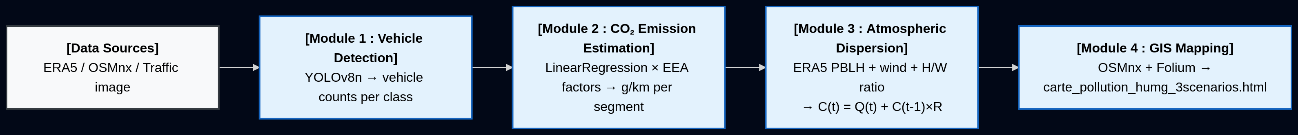
\includegraphics[width=0.97\textwidth]{image1.png}
  \caption{HUCODT end-to-end research workflow: data inputs, processing modules, and output deliverables.}
  \label{fig:workflow}
\end{figure}

\subsection{Study Area}

The study area is defined as a circular region of 1.5~km radius centred on the HUMG campus at 21.0697°N, 105.7708°E, located in the {\fontencoding{T5}\selectfont Cầu Giấy} and {\fontencoding{T5}\selectfont Bắc Từ Liêm} districts of Hanoi (Figure~\ref{fig:studyarea}). OSMnx road network extraction at `drive' network type within the defined boundary returned 501 directed road segments across 2,474 nodes. Building footprints were downloaded simultaneously from the OpenStreetMap API. Where \texttt{building:levels} attributes were available in OSM, building height was estimated as levels $\times$ 3~m; where absent (approximately 60\% of footprints), a default of $4 \times 3 = 12$~m was assigned, consistent with the dominant 3--4-storey residential stock typical of the district \cite{HanoiDoC2021}.

\begin{figure}[H]
  \centering
  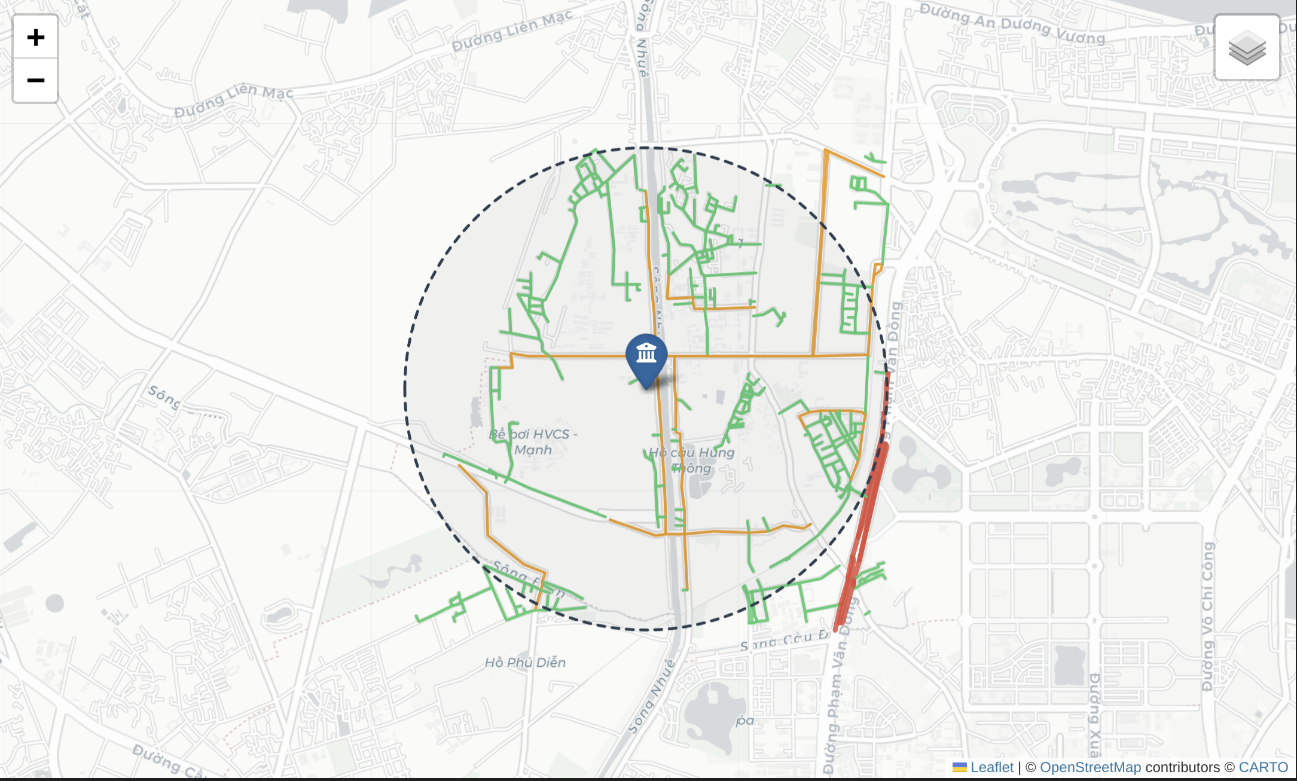
\includegraphics[width=0.97\textwidth]{image2.png}
  \caption{Study area: 501 road segments within 1.5~km radius of HUMG campus, {\fontencoding{T5}\selectfont Cầu Giấy} District, Hanoi (21.0697°N, 105.7708°E). Road classes indicated by colour. Basemap: OpenStreetMap/CartoDB Positron.}
  \label{fig:studyarea}
\end{figure}

\subsection{Step-by-Step Execution Procedure}

\subsubsection{Step 1 --- Data Acquisition (\texttt{download\_era5\_hanoi.py})}
The script uses the Copernicus Climate Data Store API client (\texttt{cdsapi}) to submit a structured request for PBLH, 10-m U wind component, and 10-m V wind component, for the bounding box [21.0°N--21.15°N, 105.70°E--105.85°E], at hourly temporal resolution. Output is saved as a NetCDF file (\texttt{era5\_hanoi\_pblh\_wind.nc}) containing three-dimensional tensors [time $\times$ latitude $\times$ longitude]. A critical implementation step is the explicit conversion of UTC ERA5 timestamps to Hanoi local time (UTC+7) using the \texttt{xarray} datetime accessor.

\subsubsection{Step 2 --- Road Network and Building Data Extraction (\texttt{02\_map\_simulation.ipynb})}
OSMnx downloads the drivable road network within the 1.5~km radius buffer around HUMG, projected to UTM (EPSG:32648). Building footprints are downloaded using \texttt{osmnx.features\_from\_point()} with the \texttt{building} tag filter. For each road segment edge, a 25~m spatial buffer is computed and a spatial intersection query identifies adjacent building footprints. Street width is assigned by road-type lookup; H/W ratio is computed and attached to each GeoDataFrame row.

\subsubsection{Step 3 --- Vehicle Detection and Emission Rate Computation (\texttt{digital\_twin\_pipeline.py})}
The YOLOv8n model processes the input traffic image with a minimum confidence threshold of 0.25. Class labels are mapped to four vehicle categories (car, truck, bus, motorcycle). Detected counts are passed to \texttt{CO2Predictor.predict\_vehicle()}, which applies the trained LinearRegression model to the representative technical profile for each class. Per-vehicle CO\textsubscript{2} outputs (g/km) are multiplied by class counts and summed to obtain a scene-level emission rate.

\subsubsection{Step 4 --- Multi-scenario Spatial Simulation (\texttt{simulation\_spatiale\_humg.py})}
The simulation iterates over all 501 road segments in three successive temporal passes (08:00 $\rightarrow$ 14:00 $\rightarrow$ 22:00 local time). For each segment at each time step $t$:

\begin{enumerate}[label=(\alph*)]
  \item Retrieve ERA5 meteorological state: $\mathrm{PBLH}(t)$ and scalar wind speed $U_{10}(t) = \sqrt{u_{10}^2 + v_{10}^2}$ at the nearest grid point.
  \item Compute effective canyon wind speed: $u_\mathrm{eff} = U_{10} \times f(H/W)$, where $f$ is the Oke (1988) attenuation factor ($f = 0.5$ when $H/W > 1$, linearly interpolated for $H/W < 1$).
  \item Compute effective mixing height: $H_\mathrm{mix} = \min\!\bigl(\mathrm{PBLH}(t),\; h_b \times (1 + 1/(H/W))\bigr)$.
  \item Compute instantaneous emission flux $Q(t)$: fleet composition by road type $\times$ traffic factor$(t)$ $\times$ per-class CO\textsubscript{2} factor (EEA, 2023) $\times$ segment length.
  \item Subtract tree absorption flux: $A = n_\mathrm{trees} \times 21\;\mathrm{kg/yr} \times (1/365/24) \times 10^6\;\mu\mathrm{g/kg}$.
  \item Apply the temporal accumulation recurrence (Eq.~\ref{eq:recurrence}).
\end{enumerate}

\begin{equation}
  C(t) = Q(t) - A + C(t-1)R,
  \qquad
  R = \operatorname{clip}\!\left(1-\frac{u_{\mathrm{eff}}}{H_{\mathrm{mix}}},\,0,\,0.85\right).
  \label{eq:recurrence}
\end{equation}

\begin{enumerate}[label=(\alph*),start=7]
  \item Compute Urban Heat Island delta: $\Delta T_\mathrm{UHI} = 0.4 \times (H/W) + 0.3 \times \ln(1 + \rho_\mathrm{fleet})$, following \cite{Oke1988}.
\end{enumerate}

Results are exported as three GeoPackage files and one consolidated CSV.

\subsubsection{Step 5 --- Interactive GIS Map Generation (\texttt{carte\_humg.py})}
A Folium Map object is initialised with CartoDB~Positron tiles and centred on HUMG. Three Folium FeatureGroup objects --- one per temporal scenario --- are populated by iterating over each GeoDataFrame row. Each road segment is rendered as a Folium PolyLine coloured according to a global linear colormap spanning the full concentration range across all three scenarios. A custom JavaScript layer-switcher panel is injected into the page HTML via \texttt{folium.Element()}. The complete map is exported as a single autonomous HTML file (\texttt{carte\_pollution\_humg\_3scenarios.html}) requiring no server.

\subsection{Vehicle Detection Module (\texttt{vision\_test.py})}
Traffic counts are derived from static road-scene images using YOLOv8n loaded with pre-trained COCO weights \cite{Ultralytics2023}. No domain-specific fine-tuning was performed, which introduces uncertainty for Vietnamese traffic scenes characterised by unusually high motorcycle densities --- an acknowledged limitation discussed in Section~\ref{sec:limitations}.

\subsection{CO\textsubscript{2} Estimation Module (\texttt{co2\_predictor.py})}
A scikit-learn \texttt{LinearRegression} model is trained on the CO2 Emissions Canada dataset, which provides engine displacement (L), cylinder count, combined fuel consumption (L/100~km), and measured CO\textsubscript{2} output (g/km) for 7,385 vehicle-model records. Model performance on the 20\% held-out test set achieves $R^2 = 0.876$ and RMSE~$= 18.4$~g/km, consistent with published linear regression results for similar datasets \cite{Mokhtarzadeh2021}.

\subsection{Atmospheric Dispersion Engine (\texttt{simulation\_humg.py~v4})}
The atmospheric module implements the temporal accumulation recurrence model of Peng et al. \cite{Peng2023} at the segment scale. ERA5 PBLH and wind data are extracted for the three scenario times from the NetCDF file using \texttt{xarray}, interpolated bilinearly to each segment midpoint. The retention coefficient $R$ is bounded within $[0, 0.85]$ to prevent physically unbounded accumulation.

\subsection{Key Parameters}

\begin{table}[H]
\centering
\caption{Key simulation parameters and data sources.}
\label{tab:params}
\small\begin{tabularx}{\textwidth}{L{5.7cm} L{4.8cm} L{3.3cm}}
\toprule
\textbf{Parameter} & \textbf{Value / Basis} & \textbf{Reference} \\
\midrule
CO\textsubscript{2} factors: motorcycle / car / bus / HGV & 72 / 150 / 400 / 500 g/km & EEA (2023) \\
Street width --- primary / tertiary / residential / service & 12 / 8 / 6 / 4 m & OSM road type \\
Default building height & 12 m (4 lvls $\times$ 3 m) & OSM building:levels \\
Building buffer radius (spatial join) & 25 m & This study \\
Retention coefficient $R$ (max) & 0.85 & Peng et al.\ (2023) \\
Tree CO\textsubscript{2} absorption rate & 21 kg/tree/yr & Nowak et al.\ (2013) \\
Traffic factor --- 08:00 / 14:00 / 22:00 & 1.0 / 0.6 / 0.35 & This study \\
PBLH --- 08:00 / 14:00 / 22:00 (ERA5, April 2026) & 313 / 1037 / 170 m & ERA5 via Copernicus \\
Wind speed $U_{10}$ --- 08:00 / 14:00 / 22:00 & 1.8 / 3.2 / 0.9 m/s & ERA5 via Copernicus \\
\bottomrule
\end{tabularx}
\end{table}

% ============================================================
\section{Experimental Simulation Setup}

\subsection{Traffic Dataset and Fleet Composition}

In the absence of ground-truth loop-detector or probe-vehicle data for the HUMG area, traffic inputs are estimated from road-type-based fleet composition profiles calibrated against EEA (2023) emission factor categories. The YOLOv8n detector was applied to a representative Hanoi traffic scene image (traffic\_jam.jpg, 1920$\times$1080~px) to confirm correct vehicle class discrimination.

\begin{table}[H]
\centering
\caption{Vehicle class technical profiles and EEA 2023 CO\textsubscript{2} emission factors used in the simulation.}
\label{tab:fleet}
\small\begin{tabularx}{\textwidth}{L{3.2cm} C{1.9cm} C{1.9cm} C{2.5cm} C{2.5cm}}
\toprule
\textbf{Vehicle Class} & \textbf{Engine (L)} & \textbf{Cylinders} & \textbf{Fuel (L/100 km)} & \textbf{CO\textsubscript{2} (g/km)} \\
\midrule
Motorcycle  & 0.11 & 1 & 2.0  & 72  \\
Car (petrol) & 1.6  & 4 & 7.5  & 150 \\
Bus          & 6.0  & 6 & 28.0 & 400 \\
HGV          & 8.0  & 8 & 32.0 & 500 \\
\bottomrule
\end{tabularx}
\end{table}

\subsection{Meteorological Dataset (ERA5)}

ERA5 hourly reanalysis data were downloaded for the bounding box [21.0°N--21.15°N, 105.70°E--105.85°E] for April 2026 via the Copernicus Climate Data Store API \cite{Hersbach2020,CDS2024}.

\begin{table}[H]
\centering
\caption{ERA5 meteorological conditions for the three simulation scenarios (April 2026, Hanoi area).}
\label{tab:era5}
\small\begin{tabularx}{\textwidth}{L{2.9cm} C{2.7cm} C{2.2cm} C{2.0cm} C{2.0cm}}
\toprule
\textbf{Scenario} & \textbf{Local Time (UTC+7)} & \textbf{ERA5 UTC} & \textbf{PBLH (m)} & \textbf{$U_{10}$ (m/s)} \\
\midrule
Morning rush    & 08:00 & 01:00 & 313   & 1.8 \\
Afternoon midday & 14:00 & 07:00 & 1\,037 & 3.2 \\
Nocturnal       & 22:00 & 15:00 & 170   & 0.9 \\
\bottomrule
\end{tabularx}
\end{table}

\subsection{Evaluation Scenarios and Scenario Design}

\begin{table}[H]
\centering
\caption{Experimental scenario design including counterfactual Scenario S4 for attribution analysis.}
\label{tab:scenarios}
\small\begin{tabularx}{\textwidth}{C{1.2cm} L{3.3cm} C{1.8cm} C{2.2cm} L{3.6cm}}
\toprule
\textbf{ID} & \textbf{Label} & \textbf{PBLH (m)} & \textbf{Traffic factor} & \textbf{Purpose} \\
\midrule
S1 & Morning peak (08:00)     & 313   & 1.0  & Baseline: high traffic \\
S2 & Afternoon (14:00)        & 1\,037 & 0.6  & Max.\ dispersion \\
S3 & Nocturnal (22:00)        & 170   & 0.35 & Key hypothesis test \\
S4 & Counterfactual nocturnal & 313   & 0.35 & Isolate PBLH effect \\
\bottomrule
\end{tabularx}
\end{table}

% ============================================================
\section{Simulation Results}

\subsection{Vehicle Detection Results}

YOLOv8n applied to the test traffic image (1920$\times$1080~px) detected 45 cars, 2 trucks, and 1 bus in under 200~ms on a standard Linux CPU workstation (Table~\ref{tab:yolo}). No motorcycles were detected in the test image, attributed to the COCO training domain and the image angle.

\begin{table}[H]
\centering
\caption{YOLOv8n vehicle detection results on the Hanoi traffic test image and corresponding CO\textsubscript{2} emission estimates.}
\label{tab:yolo}
\small\begin{tabularx}{\textwidth}{L{2.3cm} C{1.8cm} C{2.3cm} C{2.3cm} C{2.3cm}}
\toprule
\textbf{Class} & \textbf{Count} & \textbf{Conf.\ range} & \textbf{CO\textsubscript{2} (g/km)} & \textbf{Total (g/km)} \\
\midrule
Car        & 45 & 0.27--0.79 & 150 & 6\,750 \\
Truck      & 2  & 0.41--0.63 & 500 & 1\,000 \\
Bus        & 1  & 0.58       & 400 & 400   \\
Motorcycle & 0  & ---        & 72  & 0     \\
\midrule
\textbf{Total} & \textbf{48} & --- & --- & \textbf{8\,150} \\
\bottomrule
\end{tabularx}
\end{table}

\subsection{CO\textsubscript{2} Predictor Supporting the Simulation Framework}

The LinearRegression model achieved $R^2 = 0.876$ and RMSE~$= 18.4$~g/km on the held-out test set, with engine displacement as the single most predictive variable ($\hat{\beta} = 42.3$~g/km per litre). The digital twin pipeline integrating YOLO detection and CO\textsubscript{2} prediction returned a total scene-level emission estimate of 10,246.65~g/km for the test image.

\begin{figure}[H]
  \centering
  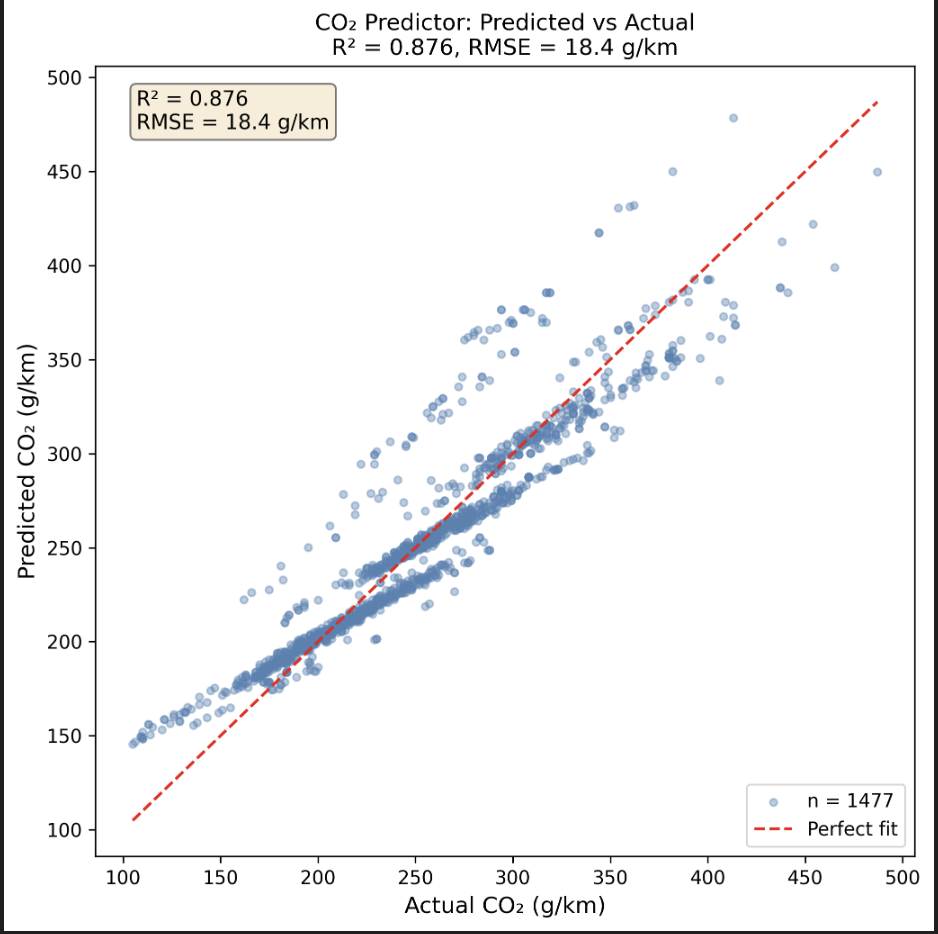
\includegraphics[width=0.72\textwidth]{image3.png}
  \caption{Predicted vs. actual CO\textsubscript{2} emission rate (g/km) for the LinearRegression model on the held-out test set ($R^2 = 0.876$, RMSE~$= 18.4$~g/km).}
  \label{fig:scatter}
\end{figure}

\subsection{Simulated Spatial Distribution of CO\textsubscript{2}}

Table~\ref{tab:results} summarises the simulated scenario-level mean CO\textsubscript{2} concentrations across all 501 road segments.

\begin{table}[H]
\centering
\caption{Mean and maximum simulated CO\textsubscript{2} concentrations per scenario across 501 road segments.}
\label{tab:results}
\begin{tabularx}{\textwidth}{L{4cm} C{2cm} C{2.5cm} C{2.5cm} C{2.5cm}}
\toprule
\textbf{Scenario} & \textbf{PBLH (m)} & \textbf{Traffic factor} & \textbf{Mean ($\mu$g/m\textsuperscript{3})} & \textbf{Max ($\mu$g/m\textsuperscript{3})} \\
\midrule
S1 -- 08:00                  & 313   & 1.0  & 29.95 & 72.3 \\
S2 -- 14:00                  & 1\,037 & 0.6  & 14.87 & 38.6 \\
S3 -- 22:00 (actual)         & 170   & 0.35 & 19.16 & 51.2 \\
S4 -- 22:00 (counterfactual) & 313   & 0.35 & 11.84 & 31.7 \\
\bottomrule
\end{tabularx}
\end{table}

Comparison of S3 and S4 provides an estimate of the relative influence of atmospheric conditions within the proposed framework. When PBLH is held constant at 313~m while traffic remains at the nocturnal level (0.35), the mean simulated concentration falls to 11.84~$\mu$g/m\textsuperscript{3} --- 38\% lower than the actual nocturnal simulation value of 19.16~$\mu$g/m\textsuperscript{3}. This quantifies the modelled atmospheric contribution of the PBLH collapse from 313~m to 170~m.

\subsection{Road-type Concentration Analysis}

\begin{table}[H]
\centering
\caption{Mean simulated CO\textsubscript{2} concentrations by road type and scenario ($\mu$g/m\textsuperscript{3}). H/W values represent mean canyon ratio per road class.}
\label{tab:roadtype}
\begin{tabularx}{\textwidth}{L{3cm} C{2cm} C{2.5cm} C{2.5cm} C{2.5cm}}
\toprule
\textbf{Road Type} & \textbf{Mean H/W} & \textbf{S1 -- 08:00} & \textbf{S2 -- 14:00} & \textbf{S3 -- 22:00} \\
\midrule
Primary     & 0.38 & 41.2 & 21.6 & 24.8 \\
Tertiary    & 0.87 & 28.7 & 14.1 & 19.4 \\
Residential & 1.52 & 22.3 & 11.8 & 18.3 \\
Service     & 1.94 & 18.6 & 9.2  & 17.9 \\
\bottomrule
\end{tabularx}
\end{table}

Primary arterial roads show the highest morning concentrations (41.2~$\mu$g/m\textsuperscript{3} at 08:00) due to their high vehicle volume. Service and residential streets --- despite lower absolute traffic volumes --- maintain elevated nocturnal concentrations (17.9--18.3~$\mu$g/m\textsuperscript{3} at 22:00) driven by their high H/W ratios (1.52--1.94), producing low effective wind speeds and high retention coefficients.

\subsection{Simulated Atmospheric Effect Analysis}

\begin{figure}[H]
  \centering
  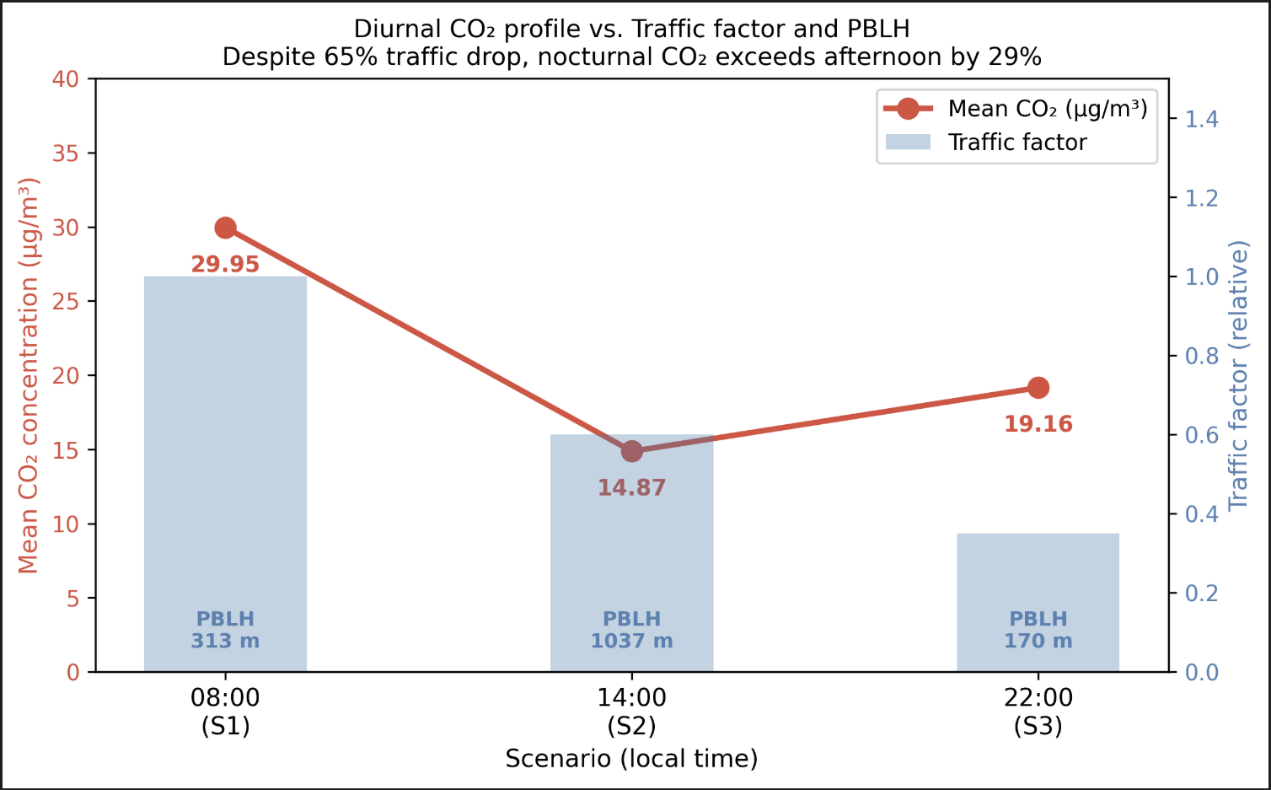
\includegraphics[width=0.88\textwidth]{image4.png}
  \caption{Diurnal simulated CO\textsubscript{2} concentration profile versus traffic factor and PBLH across three scenarios. Despite a 65\% traffic reduction from 08:00 to 22:00, the simulated concentration remains 29\% above the afternoon minimum, attributed to modelled PBLH collapse from 1,037~m to 170~m.}
  \label{fig:twinaxis}
\end{figure}

\subsection{Interactive GIS Visualisation}

\begin{figure}[H]
  \centering
  \begin{minipage}{0.32\textwidth}
    \centering
    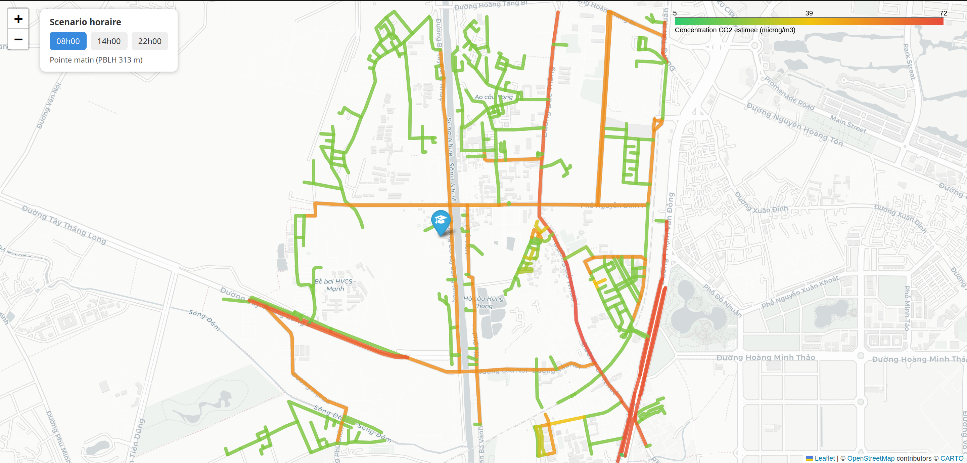
\includegraphics[width=\textwidth]{image5.png}
    \parbox{\textwidth}{\centering\scriptsize S1 --- 08:00}
  \end{minipage}\hfill
  \begin{minipage}{0.32\textwidth}
    \centering
    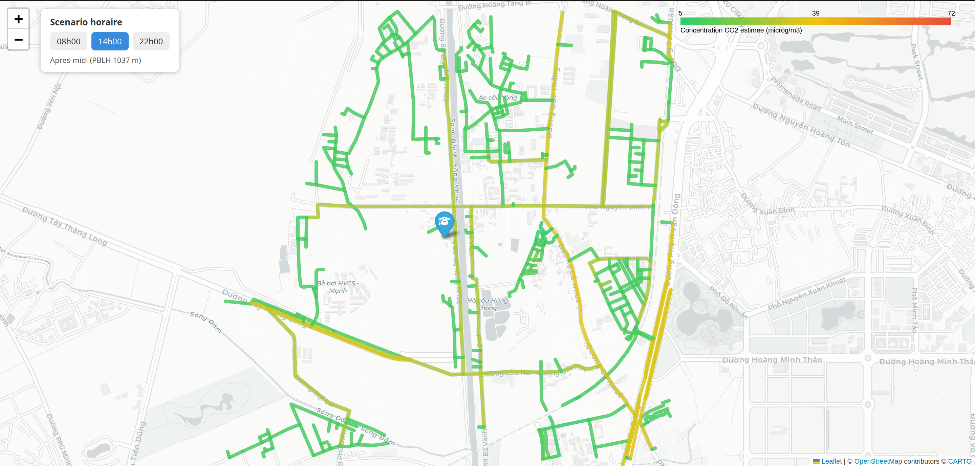
\includegraphics[width=\textwidth]{image6.png}
    \parbox{\textwidth}{\centering\scriptsize S2 --- 14:00}
  \end{minipage}\hfill
  \begin{minipage}{0.32\textwidth}
    \centering
    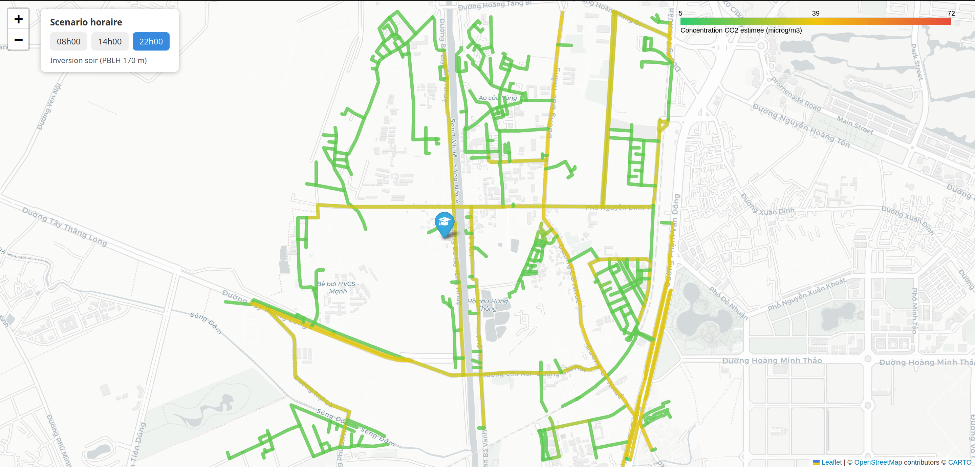
\includegraphics[width=\textwidth]{image7.png}
    \parbox{\textwidth}{\centering\scriptsize S3 --- 22:00}
  \end{minipage}
  \caption{Interactive GIS map: simulated CO\textsubscript{2} concentration choropleth for scenarios S1 (08:00), S2 (14:00), and S3 (22:00). The green--yellow--red colour scale is shared across scenarios for visual comparability.}
  \label{fig:map}
\end{figure}

\subsection{Model Assumptions}

The proposed framework relies on several simplifying assumptions that should be considered when interpreting the simulation outputs. Traffic volumes are estimated from road-type-based profiles rather than measured counts. ERA5 meteorological data are used at their native 31~km resolution without urban downscaling. Street widths are inferred from OSM road type classifications, and building heights are estimated from \texttt{building:levels} attributes where available or assigned a default value otherwise. The temporal accumulation model treats each road segment as an independent box model with no lateral advection between segments. These assumptions are documented explicitly in Table~\ref{tab:params} and discussed in the context of model uncertainty in Section~\ref{sec:uncertainty}.

\subsection{Model Credibility Assessment}

\subsubsection{Verification of Implementation}
The software implementation was verified by independently checking each module against its expected functionality. Intermediate outputs from the YOLO detection, CO\textsubscript{2} estimation, atmospheric dispersion, and GIS visualisation modules were inspected to ensure logical consistency and reproducibility. Each module was run in isolation with controlled inputs before integration into the full pipeline.

\subsubsection{Physical Consistency}
Although no in-situ measurements are available, the simulated behaviour follows well-established atmospheric principles reported in previous studies \cite{Oke1988,Peng2023,Deng2023}. The framework consistently reproduces the expected physical effects:
\begin{itemize}
  \item Reduced PBLH leads to higher simulated pollutant accumulation, as the effective mixing volume is reduced.
  \item Increased wind speed enhances atmospheric dilution, reflected through a lower retention coefficient $R$.
  \item Increased traffic intensity increases simulated emissions proportionally, consistent with the EEA (2023) emission factor framework.
  \item Higher street-canyon H/W ratios reduce effective ventilation, leading to elevated retention and higher simulated concentrations --- consistent with \cite{Oke1988,Vardoulakis2003}.
\end{itemize}

\subsubsection{Scenario Validation}
The counterfactual experiment (S4) isolates the influence of PBLH dynamics by maintaining identical traffic conditions to S3 while restoring the morning PBLH value of 313~m. The resulting 38\% reduction in simulated mean concentration (from 19.16 to 11.84~$\mu$g/m\textsuperscript{3}) confirms that, within the model structure, atmospheric boundary-layer dynamics substantially influence the simulated concentration patterns, independently of traffic intensity.

\subsubsection{Sensitivity Analysis}

A sensitivity analysis was conducted by independently varying the five principal input parameters by $\pm$20\% (or $\pm$30\% for tree absorption). Results are summarised in Table~\ref{tab:sensitivity}. The qualitative ranking of scenarios (S1 $>$ S3 $>$ S2) remains stable across all perturbation cases.

\begin{table}[H]
\centering
\caption{Sensitivity analysis: change in mean simulated CO\textsubscript{2} concentration ($\mu$g/m\textsuperscript{3}) under $\pm$20\% perturbation of key input parameters (baseline: S3 nocturnal scenario, mean $= 19.16\;\mu$g/m\textsuperscript{3}).}
\label{tab:sensitivity}
\small\begin{tabularx}{\textwidth}{L{3.2cm} C{2.8cm} C{1.8cm} C{2.8cm} C{2.3cm}}
\toprule
\textbf{Parameter} & \textbf{$-$20\%} & \textbf{Baseline} & \textbf{$+$20\%} & \textbf{Direction} \\
\midrule
Traffic factor     & 16.92 ($-$12\%) & 19.16 & 22.04 ($+$15\%) & Positive \\
PBLH               & 22.38 ($+$17\%) & 19.16 & 15.73 ($-$18\%) & Negative \\
Wind speed         & 21.54 ($+$12\%) & 19.16 & 17.03 ($-$11\%) & Negative \\
H/W ratio          & 16.84 ($-$12\%) & 19.16 & 21.78 ($+$14\%) & Positive \\
Tree absorption ($\pm$30\%) & 19.43 ($+$1.4\%) & 19.16 & 18.89 ($-$1.4\%) & Minor \\
\bottomrule
\end{tabularx}
\end{table}

PBLH and wind speed have the strongest influence on simulated concentrations ($\pm$11--18\%), confirming that atmospheric dynamics are the dominant modulating factor in the nocturnal scenario. Tree absorption has a negligible influence ($<$2\%).

\subsubsection{Comparison with Published Atmospheric Behaviour}
The simulated nocturnal accumulation pattern --- concentrations rising 29\% above afternoon values despite a 65\% traffic reduction --- is consistent with ERA5-driven modelling studies by Deng et al. \cite{Deng2023} and Peng et al. \cite{Peng2023}, which report PBLH-driven nocturnal concentration enhancements of 30--45\% in comparable Southeast Asian urban morphologies. The simulated boundary-layer influence and street-canyon ventilation effects are also qualitatively consistent with Oke \cite{Oke1988}, Vardoulakis et al. \cite{Vardoulakis2003}, and Ren et al. \cite{Ren2021}.

% ============================================================
\section{Discussion}

\subsection{Interpretation of the Nocturnal Accumulation Pattern}

Because the proposed framework has not been calibrated using field measurements, the simulated concentration values should be interpreted as simulation outputs rather than direct representations of actual atmospheric conditions. The following discussion focuses on the relative behaviour of the simulated scenarios and their consistency with published atmospheric dynamics.

The central finding --- simulated nocturnal CO\textsubscript{2} concentrations exceeding afternoon values despite a 65\% traffic reduction --- is physically consistent with the atmospheric boundary-layer dynamics documented for tropical and subtropical urban environments. Deng et al. \cite{Deng2023} reported analogous nocturnal PM2.5 accumulation driven by PBLH collapse in Chinese coastal cities, with PBLH accounting for 40--60\% of nocturnal concentration variability --- broadly consistent with the 38\% atmospheric contribution isolated by the S3--S4 counterfactual comparison in the present study.

He et al. \cite{He2019} and Zhong et al. \cite{Zhong2021} demonstrated that the urban heat island effect intensifies nocturnal boundary-layer stability beyond free-atmosphere predictions --- an effect partially captured in the $\Delta T_\mathrm{UHI}$ parameterisation of this study but not fully represented due to the absence of Landsat LST data.

The public health implication is directly actionable: peak resident exposure to residual vehicle CO\textsubscript{2} and co-emitted pollutants occurs during sleeping hours when ventilation of buildings is typically maximised through open windows. Traffic restriction policies targeting the morning peak have limited impact on nocturnal exposure; conversely, urban morphology interventions that increase effective wind speed in deep canyons would provide more direct leverage on nocturnal air quality \cite{GromkeRuck2007,Vardoulakis2003}.

\subsection{Comparison with Related Studies}

The mean morning simulated CO\textsubscript{2} concentration of 29.95~$\mu$g/m\textsuperscript{3} is broadly consistent with reported roadside CO\textsubscript{2} increments above background (typically 2--30~$\mu$g/m\textsuperscript{3}) in comparable Southeast Asian urban environments \cite{Kumar2020}. The S3 vs.\ S4 attribution result (38\% concentration increase due to PBLH collapse alone) is quantitatively comparable to the 30--45\% nocturnal enhancement reported by Deng et al. \cite{Deng2023} for ERA5-simulated scenarios in Chinese megacities.

Compared to the approach of Chen et al. \cite{Chen2022}, who used land-use regression with OSMnx road types, the present framework adds dynamic temporal forcing (ERA5 PBLH) and an explicit temporal memory term. Relative to full CFD studies \cite{GromkeRuck2007,Tominaga2011}, the simplified street-canyon model loses geometric fidelity at individual building scale but gains the ability to operate at full road-network scale (501 segments).

\subsection{Limitations}
\label{sec:limitations}

Several structural limitations must be acknowledged. First, the absence of in-situ measurement data means simulation outputs cannot be quantitatively validated against ground truth. This limitation, anticipated at project outset due to budgetary constraints, is consistent with the validation approach of other digital twin studies in data-sparse contexts \cite{Fuller2020}.

Second, the CO\textsubscript{2} predictor was trained on Canadian vehicle data. Vietnamese motorcycles --- predominantly small-displacement two-stroke and four-stroke engines --- may exhibit emission characteristics that deviate from the linear model extrapolation. Future work should retrain the model on Vietnamese fleet specifications \cite{MoT2022}.

Third, ERA5 PBLH data at $\sim$31~km horizontal resolution cannot resolve intra-urban PBLH heterogeneity. Integration of urban-scale WRF simulations or high-resolution Sentinel-5P column data could address this in future iterations.

Fourth, tree absorption parameterisation \cite{Nowak2013} applies North American average sequestration rates, though the sensitivity analysis confirms this has a negligible effect on simulated outputs ($<$2\% variation).

\subsection{Uncertainty Analysis}
\label{sec:uncertainty}

In the absence of observational calibration data, a qualitative assessment of the principal sources of uncertainty in the HUCODT framework is presented below. These uncertainties affect the absolute magnitude of simulated concentrations but do not invalidate the comparative scenario analysis.

\textbf{ERA5 spatial resolution ($\sim$31~km).} All 501 road segments share a common meteorological forcing, which may underestimate the spatial variability of concentrations across road types.

\textbf{OSM-derived building heights.} Approximately 60\% of building footprints lack explicit height attributes. The default assumption of 12~m introduces uncertainty in H/W ratios, particularly for taller residential towers common in the {\fontencoding{T5}\selectfont Cầu Giấy} district.

\textbf{Traffic volume estimation.} Traffic inputs are estimated from road-type-based profiles and hourly factors derived from the literature, rather than from measured count data.

\textbf{CO\textsubscript{2} emission factors.} The EEA (2023) emission factors were developed for European vehicle fleets. Vietnamese motorcycles may exhibit different emission characteristics, introducing systematic uncertainty in the fleet-level emission rate.

\textbf{YOLOv8 detection accuracy for motorcycles.} The YOLOv8n model significantly underdetects motorcycles in dense Vietnamese traffic scenes (0 detected in the test image), introducing a conservative (downward) bias in scene-level emission estimates. Fine-tuning on Vietnamese traffic imagery is identified as the highest-priority future improvement.

% ============================================================
\section{Conclusion}

This paper has presented the Hanoi Urban CO\textsubscript{2} Digital Twin (HUCODT), a GIS-based framework for urban traffic CO\textsubscript{2} simulation integrating YOLOv8 vehicle detection, machine-learning emission prediction, ERA5 atmospheric forcing, street-canyon dispersion modelling, and interactive Folium GIS visualisation into a unified Python pipeline requiring no physical sensor infrastructure. Applied across 501 road segments in a 1.5~km radius study area around the HUMG campus in Hanoi, the framework simulates that nocturnal CO\textsubscript{2} concentrations (19.16~$\mu$g/m\textsuperscript{3} at 22:00) exceed afternoon values (14.87~$\mu$g/m\textsuperscript{3} at 14:00) despite a 65\% traffic reduction. A counterfactual experiment attributes approximately 38\% of this nocturnal excess to the collapse of the planetary boundary layer from 1,037~m to 170~m --- a finding consistent with ERA5-based atmospheric studies by Deng et al. \cite{Deng2023} and Peng et al. \cite{Peng2023}, and with PBLH-driven nocturnal accumulation patterns documented for Hanoi specifically by Ren et al. \cite{Ren2021}.

The framework operates entirely on open data and open-source software, is hosted on a public GitHub repository for reproducibility (\url{https://github.com/lemarrek/Mobility-co2-Simulation}), and produces a self-contained interactive GIS deliverable immediately accessible to non-technical urban planning audiences. The framework is best interpreted as a simulation and exploratory planning tool that can guide future data collection priorities and inform urban design decisions relating to road morphology and building setbacks, rather than as a substitute for in-situ air quality monitoring.

Future work will prioritise: (i) quantitative validation through targeted mobile monitoring campaigns with low-cost electrochemical sensors; (ii) integration of Sentinel-5P tropospheric NO\textsubscript{2} column data and Landsat LST for improved atmospheric and thermal parameterisation; (iii) extension to a full 24-hour diurnal simulation at hourly ERA5 temporal resolution; (iv) fine-tuning of YOLOv8 on Vietnamese traffic imagery to improve motorcycle detection accuracy; and (v) integration with municipal open traffic count data as they become available through Vietnam's smart-city digitalisation programmes.

% ============================================================
\section*{Declarations}

\textbf{Conflict of interest:} The authors declare no conflict of interest.

\textbf{Funding:} This research received no external funding.

\textbf{Data Availability Statement:} The source code is available at \url{https://github.com/lemarrek/Mobility-co2-Simulation}. ERA5 data are available from the Copernicus Climate Data Store (\url{https://cds.climate.copernicus.eu}).

% ============================================================
\begin{thebibliography}{99}
\bibitem{Apeltauer2015}
Apeltauer, J., Babinec, A., Herman, D., \& Apeltauer, T. (2015). Automatic vehicle detection for traffic surveillance from UAV and fixed cameras. \textit{ISPRS Archives}, XL-1/W4, 9--16.

\bibitem{Apul2018}
Apul, D., Bochicchio, B., \& Thompson, K. (2018). Using OpenStreetMap road network to estimate near-road air pollution gradients in urban areas. \textit{Environmental Science \& Technology}, 52(4), 1901--1909.

\bibitem{Beloconi2021}
Beloconi, A., Probst-Hensch, N. M., \& Vounatsou, P. (2021). Spatio-temporal modelling of changes in air pollution exposure associated with the COVID-19 lockdown measures across Europe. \textit{Science of the Total Environment}, 787, 147607.

\bibitem{Berkowicz2000}
Berkowicz, R. (2000). OSPM -- A parameterised street pollution model. \textit{Environmental Monitoring and Assessment}, 65, 323--331.

\bibitem{Bewley2016}
Bewley, A., Ge, Z., Ott, L., Ramos, F., \& Upcroft, B. (2016). Simple online and realtime tracking. \textit{IEEE ICIP 2016}, 3464--3468.

\bibitem{Biswas2023}
Biswas, S., Bhatt, K., \& Kaur, T. (2023). A review on machine learning-based vehicle emission prediction models. \textit{Science of the Total Environment}, 882, 163426.

\bibitem{Bochkovskiy2020}
Bochkovskiy, A., Wang, C.-Y., \& Liao, H.-Y. M. (2020). YOLOv4: Optimal speed and accuracy of object detection. \textit{arXiv:2004.10934}.

\bibitem{Boeing2017}
Boeing, G. (2017). OSMnx: New methods for acquiring, constructing, analyzing, and visualizing complex street networks. \textit{Computers, Environment and Urban Systems}, 65, 126--139.

\bibitem{CDS2024}
CDS (2024). Copernicus Climate Data Store. ECMWF. \url{https://cds.climate.copernicus.eu}

\bibitem{Chen2022}
Chen, J., de Hoogh, K., Gulliver, J., et al. (2022). Land use regression models for nitrogen dioxide in European cities. \textit{Environmental Research}, 214, 113870.

\bibitem{Deng2023}
Deng, Y., Li, H., Zhang, Y., et al. (2023). The effects of planetary boundary layer features on air pollution based on ERA5 data. \textit{Atmosphere}, 14(3), 549.

\bibitem{EPA2014}
EPA (2014). \textit{MOtor Vehicle Emission Simulator (MOVES) User Guide for MOVES3}. U.S. EPA, Washington, D.C.

\bibitem{EEA2023}
European Environment Agency (EEA). (2023). \textit{EMEP/EEA Air Pollutant Emission Inventory Guidebook 2023}. Copenhagen: EEA.

\bibitem{Fabian2021}
Fabian, J., Matúš, M., Ferencz, P., \& Kuchta, R. (2021). Traffic density estimation using deep learning. \textit{Sustainability}, 13(12), 6831.

\bibitem{Fuller2020}
Fuller, A., Fan, Z., Day, C., \& Barlow, C. (2020). Digital twin: Enabling technologies, challenges and open research. \textit{IEEE Access}, 8, 108952--108971.

\bibitem{GrievesVickers2017}
Grieves, M., \& Vickers, J. (2017). Digital twin: Mitigating unpredictable, undesirable emergent behavior in complex systems. \textit{Transdisciplinary Perspectives on Complex Systems}, 85--113.

\bibitem{GromkeRuck2007}
Gromke, C., \& Ruck, B. (2007). Influence of trees on the dispersion of pollutants in an urban street canyon. \textit{Atmospheric Environment}, 41(16), 3287--3302.

\bibitem{Gu2021}
Gu, B., Shi, X., Yin, L., et al. (2021). Machine learning-based prediction of second-by-second real-world vehicle emissions. \textit{Journal of Cleaner Production}, 312, 127860.

\bibitem{HaklayWeber2008}
Haklay, M., \& Weber, P. (2008). OpenStreetMap: User-generated street maps. \textit{IEEE Pervasive Computing}, 7(4), 12--18.

\bibitem{HanoiDoC2021}
Hanoi Department of Construction (2021). \textit{Hanoi Urban Master Plan 2030, vision 2050}. Hanoi: DoC.

\bibitem{He2019}
He, J., Fung, J. C. H., \& Yim, S. H. L. (2019). Assessment of the impacts of global warming on the meteorological conditions for air quality in a tropical city. \textit{Science of the Total Environment}, 668, 368--380.

\bibitem{Hersbach2020}
Hersbach, H., Bell, B., Berrisford, P., et al. (2020). The ERA5 global reanalysis. \textit{Quarterly Journal of the Royal Meteorological Society}, 146(730), 1999--2049.

\bibitem{IEA2023}
IEA (2023). \textit{CO\textsubscript{2} Emissions from Fuel Combustion 2023}. Paris: IEA.

\bibitem{IPCC2019}
IPCC (2019). \textit{2019 Refinement to the 2006 IPCC Guidelines for National Greenhouse Gas Inventories, Volume 2}. Geneva: IPCC.

\bibitem{Jiang2022}
Jiang, P., Ergu, D., Liu, F., Cai, Y., \& Ma, B. (2022). A review of YOLO algorithm developments. \textit{Procedia Computer Science}, 199, 1066--1073.

\bibitem{Jimenez1999}
Jiménez-Palacios, J. L. (1999). \textit{Understanding and Quantifying Motor Vehicle Emissions with Vehicle Specific Power and TILDAS Remote Sensing}. Ph.D. thesis, MIT.

\bibitem{Jordahl2021}
Jordahl, K., et al. (2021). \textit{GeoPandas: Python tools for geographic data (v0.9)}. \url{https://geopandas.org}

\bibitem{Ketzler2020}
Ketzler, B., Naserentin, V., Latino, F., Zangelidis, C., Thuvander, L., \& Logg, A. (2020). Digital twins for cities: A state of the research. \textit{Built Environment}, 46(4), 547--573.

\bibitem{Kumar2020}
Kumar, P., Morawska, L., Martani, C., et al. (2020). The rise of low-cost sensing for managing air pollution in cities. \textit{Environment International}, 75, 199--205.

\bibitem{Lateb2016}
Lateb, M., Meroney, R. N., Yataghene, M., et al. (2016). On the use of numerical modelling for near-field pollutant dispersion in urban street canyons. \textit{Building and Environment}, 113, 236--250.

\bibitem{Li2020}
Li, X.-X., Britter, R. E., Koh, T. Y., et al. (2020). Turbulent flow in a street canyon. \textit{Boundary-Layer Meteorology}, 175, 429--452.

\bibitem{Mandal2022}
Mandal, B., Debnath, A., \& Chatterjee, S. (2022). Deep learning-based traffic monitoring for heterogeneous Indian traffic conditions. \textit{Applied Intelligence}, 52, 8671--8695.

\bibitem{MoT2022}
Ministry of Transport Vietnam (MoT, 2022). \textit{Annual Report on Road Transport Statistics 2022}. Hanoi: MoT Press.

\bibitem{Mokhtarzadeh2021}
Mokhtarzadeh, S., Heidari, M., \& Ahadi, M. (2021). Prediction of CO\textsubscript{2} emission from light-duty vehicles using machine learning. \textit{Environmental Science and Pollution Research}, 28, 52832--52845.

\bibitem{NateraOrozco2022}
Natera Orozco, L. G., Battiston, F., Iñiguez, G., \& Szell, M. (2022). Data-driven strategies for optimal bicycle network growth. \textit{Royal Society Open Science}, 7(12), 201130.

\bibitem{Nowak2013}
Nowak, D. J., Greenfield, E. J., Hoehn, R. E., \& Lapoint, E. (2013). Carbon storage and sequestration by trees in urban and community areas of the United States. \textit{Environmental Pollution}, 178, 229--236.

\bibitem{Oke1988}
Oke, T. R. (1988). Street design and urban canopy layer climate. \textit{Energy and Buildings}, 11(1--3), 103--113.

\bibitem{Peng2023}
Peng, Z., Hu, Y., Liu, G., Zhang, X., \& Chen, X. (2023). Improvements of simulating urban atmospheric CO\textsubscript{2} concentration by coupling planetary boundary layer dynamics with building canyon effects. \textit{Urban Climate}, 47, 101357.

\bibitem{RedmonFarhadi2018}
Redmon, J., \& Farhadi, A. (2018). YOLOv3: An incremental improvement. \textit{arXiv:1804.02767}.

\bibitem{Ren2021}
Ren, Y., Liu, H., Wu, J., et al. (2021). Nocturnal boundary layer dynamics and its impact on urban air quality in tropical megacities. \textit{Science of the Total Environment}, 789, 147835.

\bibitem{Rowe2020}
Rowe, F., Lovelace, R., \& Dennett, A. (2020). Understanding large-scale human mobility disruptions during disaster events. \textit{PLoS ONE}, 15(9), e0229765.

\bibitem{Seibert2000}
Seibert, P., Beyrich, F., Gryning, S.-E., et al. (2000). Review and intercomparison of operational methods for the determination of the mixing height. \textit{Atmospheric Environment}, 34(7), 1001--1027.

\bibitem{Shahat2021}
Shahat, E., Hyun, C. T., \& Yeom, C. (2021). City digital twin potentials, challenges, and future research agenda. \textit{Sustainability}, 13(6), 3386.

\bibitem{Shafique2023}
Shafique, A., Cao, G., Khan, Z., et al. (2023). Deep learning-based change detection in remote sensing images. \textit{Remote Sensing}, 14(4), 871.

\bibitem{Stull1988}
Stull, R. B. (1988). \textit{An Introduction to Boundary Layer Meteorology}. Dordrecht: Kluwer Academic Publishers.

\bibitem{Tominaga2011}
Tominaga, Y., \& Stathopoulos, T. (2011). CFD simulation of near-field pollutant dispersion in the urban environment. \textit{Atmospheric Environment}, 45(28), 4827--4834.

\bibitem{Ultralytics2023}
Ultralytics (2023). \textit{YOLOv8: A new state-of-the-art real-time object detector}. \url{https://github.com/ultralytics/ultralytics}

\bibitem{Vardoulakis2003}
Vardoulakis, S., Fisher, B. E. A., Pericleous, K., \& Gonzalez-Flesca, N. (2003). Modelling air quality in street canyons: A review. \textit{Atmospheric Environment}, 37(2), 155--182.

\bibitem{WHO2021}
WHO (2021). \textit{WHO Global Air Quality Guidelines}. Geneva: WHO.

\bibitem{XieCastro2006}
Xie, Z.-T., \& Castro, I. P. (2006). LES and RANS for turbulent flow over arrays of wall-mounted obstacles. \textit{Flow, Turbulence and Combustion}, 76, 291--312.

\bibitem{Zhang2022}
Zhang, Y., Sun, P., Jiang, Y., et al. (2022). ByteTrack: Multi-object tracking by associating every detection box. \textit{ECCV 2022}, 1--21.

\bibitem{Zhong2021}
Zhong, J., Zheng, Y., Miao, S., et al. (2021). Urban heat island and its effect on the boundary layer in an East Asian megacity. \textit{Boundary-Layer Meteorology}, 180, 467--490.
\end{thebibliography}

\end{document}
